% Conditional Strategies I -- timing risk: volatility is predictable, returns mostly are not, and when that pays.
% Figures and every number quoted here come from conditional_strategies_figures.py
% Companion notebook: chapters/Finance/L14_ConditionalStrategiesI_AI.ipynb (exercises 1-5 in class, the challenge is homework)
% Structure: content first, then one slide per notebook exercise, then takeaways.
% The challenge answer (momentum capped at 2, 1963-2026) must not appear here: this PDF is public.
\documentclass[aspectratio=169,10pt]{beamer}
\usetheme{default}
\usecolortheme{default}

\usepackage{graphicx}
\usepackage{adjustbox}
\usepackage{amsmath}
\usepackage{amssymb}
\usepackage{booktabs}
\usepackage{array}
\usepackage{tikz}
\usetikzlibrary{arrows.meta,positioning,calc,decorations.pathreplacing}
\usepackage{appendixnumberbeamer}  % Exclude appendix from slide count

\setbeamertemplate{navigation symbols}{}
\setbeamertemplate{items}[circle]

% Footline: Author, Event (Year) on left; page/total on right
\setbeamertemplate{footline}{
  \hbox{%
    \begin{beamercolorbox}[wd=.5\paperwidth,ht=2.5ex,dp=1ex,left]{author in head/foot}%
      \hspace*{2ex}\insertshortauthor, \insertshortinstitute\ (\insertdate)
    \end{beamercolorbox}%
    \begin{beamercolorbox}[wd=.5\paperwidth,ht=2.5ex,dp=1ex,right]{date in head/foot}%
      \insertframenumber/\inserttotalframenumber\hspace*{2ex}
    \end{beamercolorbox}%
  }
}

% Highlight boxes
\setbeamercolor{box1}{bg=red!12,fg=black}

% A poll option: {colour}{letter and choice}
\newcommand{\pollbox}[2]{\tikz\node[draw=#1!65!black, fill=#1!10, rounded corners=4pt, minimum width=3.7cm,
                                   minimum height=1.0cm, align=center, font=\normalsize]{#2};}
\newcolumntype{P}[1]{>{\raggedright\arraybackslash}p{#1}}

\title{Conditional Strategies I}
\subtitle{Timing risk}
\author[A. Moreira]{Alan Moreira}
\institute[Data-Driven Investing]{NYU Stern --- Data-Driven Investing}
\date{Fall 2026}

\begin{document}

\begin{frame}
\titlepage
\end{frame}

%================================================================== INTRODUCTION
\begin{frame}{Your risk is not constant, even if your position is}
\vskip 6pt
\begin{itemize}
\item In a typical month the market's volatility is about 11\% a year. In March 2020 it was \textcolor{red}{93\%}.
\vskip 8pt
\item Hold the same dollars through that and you carry eight times the risk you signed up for
\vskip 8pt
\item A manager with a volatility target or a risk budget would have cut. Is that only risk control, or does it also earn a better Sharpe ratio?
\vskip 8pt
\item Today: when holding less in volatile times pays, for which factors, and what it costs
\end{itemize}
\vskip 14pt
\begin{beamercolorbox}[rounded=true,sep=7pt,center]{box1}
You do not need to forecast returns. You need to forecast risk, and the bet that returns do not rise to pay for it.
\end{beamercolorbox}
\end{frame}

\begin{frame}{The formula has two parts that can move}
\[ x_{t} \;=\; \frac{1}{\gamma}\,\frac{\mu_{t}}{\sigma_{t}^{2}} \]
{\small $x_{t}$: the weight on the asset this month \quad $\mu_{t}$, $\sigma_{t}^{2}$: its expected excess return and variance this month, as seen at the start}
\vskip 6pt
\begin{itemize}
\item \emph{Capital Allocation} held $\mu$ and $\sigma$ fixed. In practice both change over time.
\vskip 6pt
\item Today: let $\sigma_{t}$ move, and hold $\mu$ fixed. \emph{Next class}: let $\mu_{t}$ move.
\vskip 6pt
\item You saw one case already: volatility-managed momentum, in \emph{Momentum}. Is that a momentum story, or general?
\end{itemize}
\vskip 10pt
\begin{beamercolorbox}[rounded=true,sep=7pt,center]{box1}
Forecasting $\sigma$ is easy. Forecasting $\mu$ is hard. That asymmetry is the whole idea.
\end{beamercolorbox}
\end{frame}

%================================================================== MEASURING RISK
\begin{frame}{Volatility comes in waves}
\begin{center}
\adjustbox{max width=\textwidth, max height=0.58\textheight}{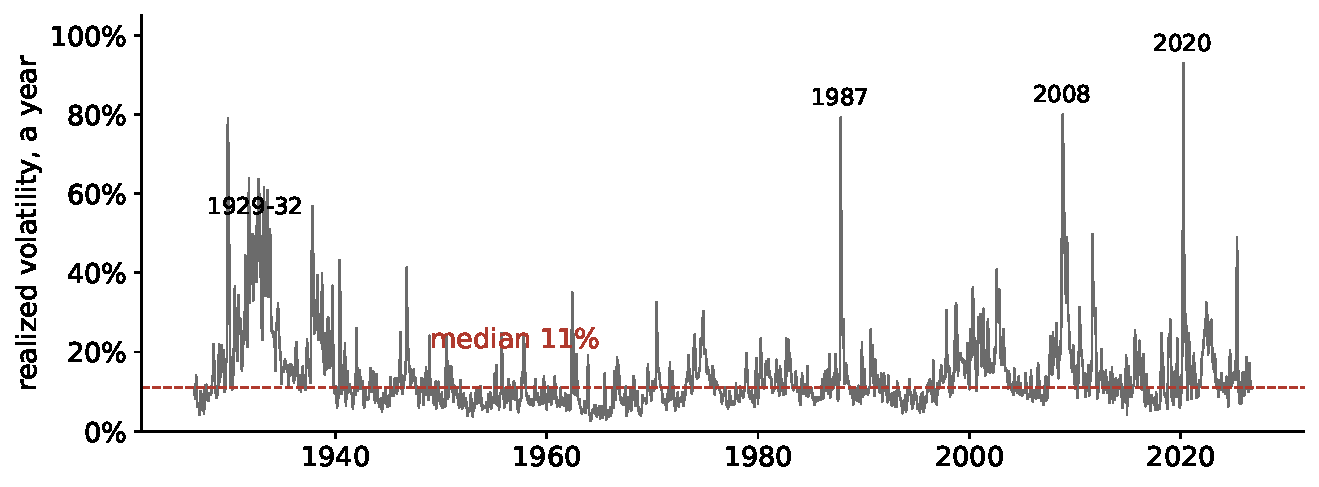
\includegraphics{figures/cs_vol_history.pdf}}
\end{center}
\begin{itemize}
\item The market, 1926--2026. Each month's volatility from its daily returns: the median is 11\% a year
\vskip 4pt
\item Spikes to about 80\% in 1929--32, 1987 and 2008, and to \textcolor{red}{93\%} in March 2020
\vskip 4pt
\item And they fade: a calm month tends to follow a calm month, a wild one a wild one
\end{itemize}
\end{frame}

\begin{frame}[label=rv]{Measuring it: realized variance}
\[ \text{RV}_{t} \;=\; \sum_{d=1}^{N_{t}} \left(r_{d} - \bar r_{t}\right)^{2} \qquad\qquad \hat\sigma_{t} \;=\; \sqrt{12 \cdot \text{RV}_{t}} \]
{\small $r_{d}$: the return on trading day $d$ of month $t$ \quad $N_{t}$: about 21 days \quad $\bar r_{t}$: their average \quad $\hat\sigma_{t}$: volatility, a year}
\vskip 8pt
\begin{itemize}
\item What the formula needs is \emph{next} month's variance, $\sigma^{2}_{t+1}$, as you see it today
\vskip 6pt
\item $\text{RV}_{t}$ is a simple proxy for it: use this month's risk as the forecast of next month's
\vskip 6pt
\item It works because volatility persists: the correlation of log $\text{RV}$ with last month's is 0.71, and still 0.51 six months later
\end{itemize}
\vskip 10pt
\begin{beamercolorbox}[rounded=true,sep=7pt,center]{box1}
Any better forecast of next month's variance can replace it
\end{beamercolorbox}
\end{frame}

\begin{frame}{Volatility forecasts itself. Returns do not.}
\begin{center}
\adjustbox{max width=\textwidth, max height=0.58\textheight}{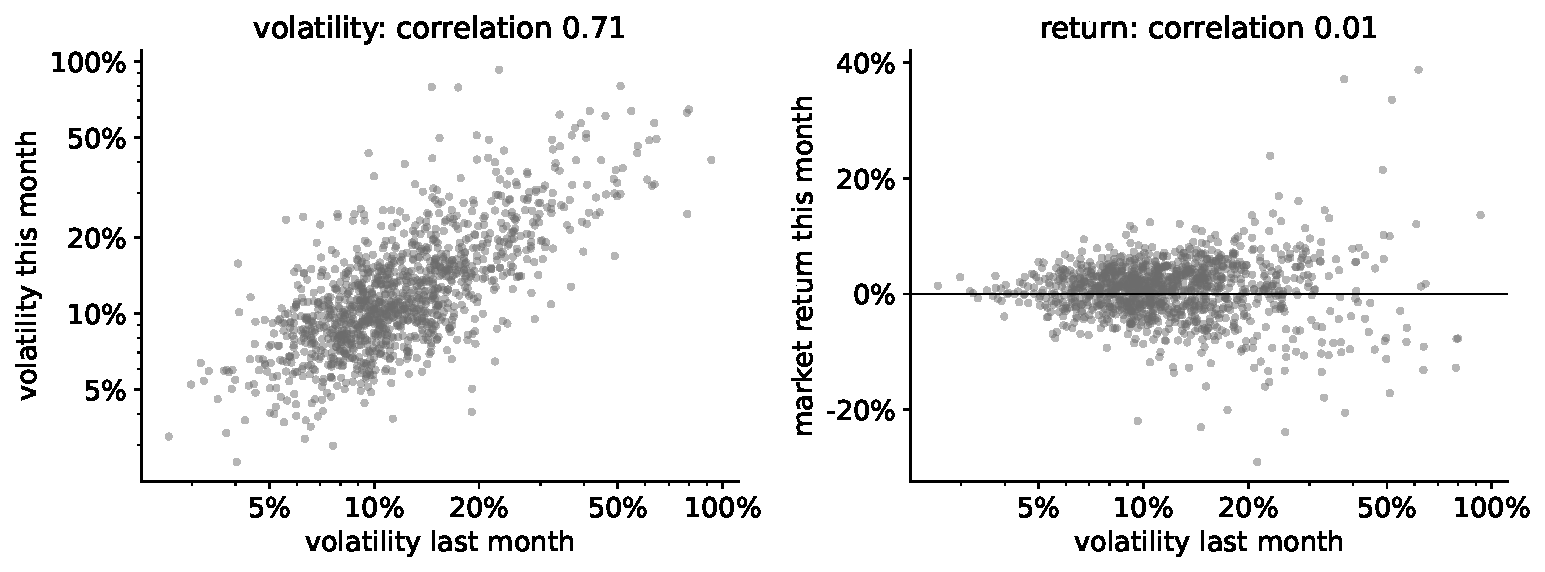
\includegraphics{figures/cs_persist.pdf}}
\end{center}
\begin{itemize}
\item Last month's volatility explains \textcolor{red}{half} of this month's (in logs, $R^{2}=0.50$)
\vskip 4pt
\item It explains none of this month's return ($R^{2}=0.00$)
\vskip 4pt
\item From \emph{Backtesting}: a mean needs decades to learn, a volatility a few weeks
\end{itemize}
\end{frame}

\begin{frame}{Can you beat last month's RV?}
\vskip 2pt
\begin{center}
\renewcommand{\arraystretch}{1.3}
\begin{tabular}{lcccc}
\toprule
 & \multicolumn{2}{c}{market, 1927--2026} & \multicolumn{2}{c}{UMD, 1964--2026} \\
forecast of next month's variance & $R^{2}$ & managed Sharpe & $R^{2}$ & managed Sharpe \\
\midrule
RV last month & 0.51 & 0.51 & 0.64 & 0.91 \\
RV, average of the last 3 months & 0.49 & 0.45 & 0.63 & \textcolor{red}{0.98} \\
RV, average of the last 12 months & 0.42 & 0.51 & 0.46 & 0.88 \\
EWMA of daily squared returns & \textcolor{red}{0.54} & 0.48 & \textcolor{red}{0.69} & 0.94 \\
\bottomrule
\end{tabular}
\end{center}
{\small $R^{2}$: of log variance next month on the forecast. EWMA: RiskMetrics, $\lambda = 0.94$. Buy and hold: 0.45 and 0.51.}
\vskip 8pt
\begin{itemize}
\item A better forecast helps a little, and not always: the best $R^{2}$ is not the best Sharpe ratio
\vskip 4pt
\item Other candidates: GARCH models, implied volatility (VIX, from 1990), intraday returns
\vskip 4pt
\item Last month's RV is crude, and hard to beat by much. That is why everyone starts there.
\end{itemize}
\end{frame}

%================================================================== WHEN IT PAYS
\begin{frame}[label=when]{When does holding less in volatile times pay?}
Suppose the expected return rises with the variance: $\;\mu_{t} = a + b\,\sigma_{t}^{2}$
\[ x_{t} \;=\; \frac{1}{\gamma}\,\frac{a + b\,\sigma_{t}^{2}}{\sigma_{t}^{2}} \;=\; \frac{1}{\gamma}\left(\frac{a}{\sigma_{t}^{2}} + b\right) \]
\vskip 4pt
\begin{center}
\renewcommand{\arraystretch}{1.4}
\begin{tabular}{lll}
\toprule
if & then & so \\
\midrule
$b = 0$: the return does not rise with risk & $x_{t} \propto 1/\sigma_{t}^{2}$ & time the risk, fully \\
$a = 0$: the return rises one for one & $x_{t}$ constant & no point timing \\
\bottomrule
\end{tabular}
\end{center}
\vskip 8pt
\begin{itemize}
\item It is an empirical question: after a volatile month, does the return rise enough to pay for the extra risk?
\end{itemize}
\end{frame}

\begin{frame}{Sort the months by last month's volatility}
\begin{center}
\adjustbox{max width=\textwidth, max height=0.56\textheight}{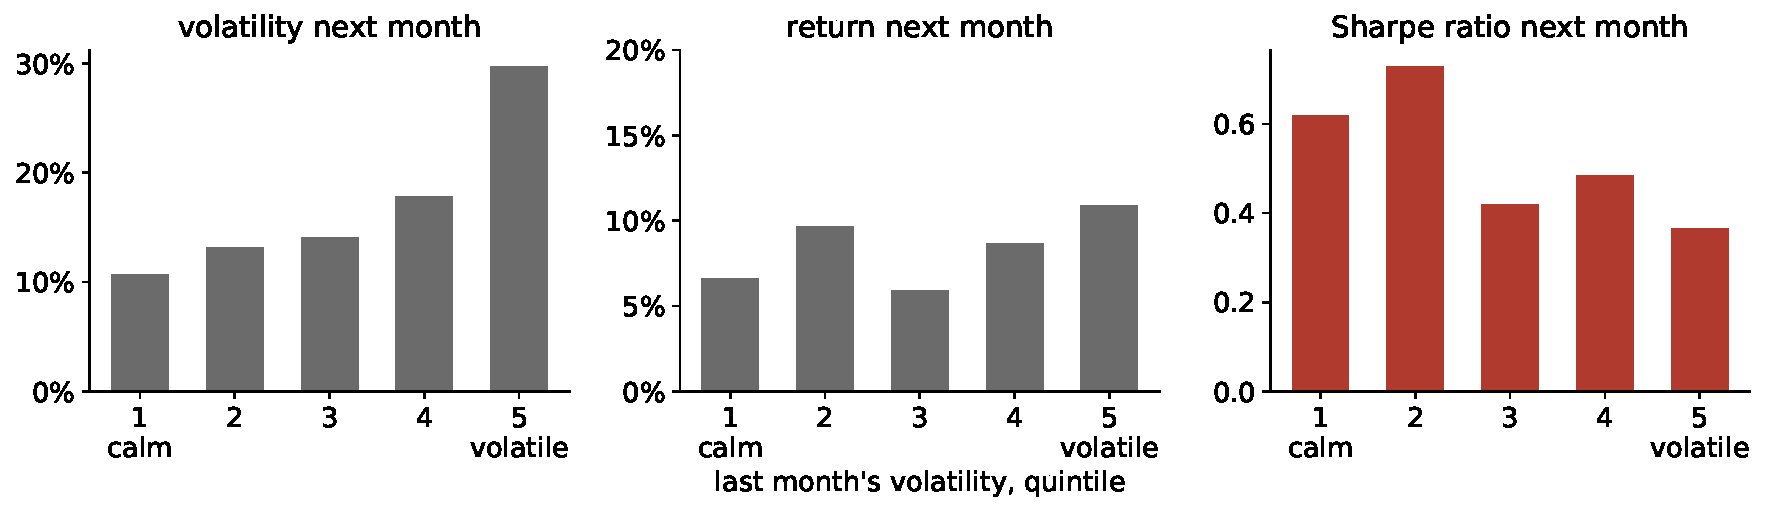
\includegraphics{figures/cs_sort_market.pdf}}
\end{center}
\begin{itemize}
\item The market, 1926--2026. After the most volatile months, volatility is nearly three times higher: 11\% to \textcolor{red}{30\%}
\vskip 4pt
\item The return does not keep up: 7\% to 11\%, with no clear pattern in between
\vskip 4pt
\item So the Sharpe ratio falls, from 0.62 after the calmest months to \textcolor{red}{0.37}. Closer to $b = 0$ than to $a = 0$.
\end{itemize}
\end{frame}

\begin{frame}[label=managed]{The strategy: hold less after a volatile month}
\[ r^{\sigma}_{t} \;=\; \frac{c}{\text{RV}_{t-1}}\; r_{t} \qquad\qquad c \;\text{ such that }\; \operatorname{sd}(r^{\sigma}) = \operatorname{sd}(r) \]
\vskip 2pt
\begin{itemize}
\item $\text{RV}_{t-1}$: last month's realized variance, known before this month starts
\vskip 6pt
\item $c$: one constant. It sets the size, not the Sharpe ratio
\vskip 6pt
\item Same volatility, so compare Sharpe ratios, or regress and read the alpha:
\[ r^{\sigma}_{t} \;=\; \alpha + \beta\, r_{t} + \varepsilon_{t} \]
\item Barroso and Santa-Clara (2015) for momentum; Moreira and Muir (2017) across factors
\end{itemize}
\vskip 6pt
\begin{beamercolorbox}[rounded=true,sep=7pt,center]{box1}
No return forecast anywhere. Only a volatility forecast, and the bet that $b$ is small.
\end{beamercolorbox}
\hfill \hyperlink{appendix_rv}{\beamerbutton{Details}}
\end{frame}

\begin{frame}{How often to rebalance, and on how much history}
\begin{center}
\renewcommand{\arraystretch}{1.12}
\adjustbox{max width=0.92\textwidth}{\begin{tabular}{llccc}
\toprule
rebalance & variance of the last & market & UMD & trades a year, market \\
\midrule
every day & 5 days & \textcolor{red}{0.05} & 0.68 & \\
every day & 21 days & 0.45 & 0.94 & 28 \\
every week & 21 days & 0.46 & 0.86 & 16 \\
every month & 21 days & 0.45 \;(0.41--0.50) & 0.85 \;(0.77--0.90) & 9 \\
every quarter & 21 days & 0.44 \;(0.38--0.50) & 0.85 \;(0.75--0.94) & 3 \\
every six months & 21 days & 0.44 \;(0.31--0.52) & 0.80 \;(0.73--0.85) & 1.5 \\
\bottomrule
\end{tabular}}
\end{center}
{\small Sharpe ratios, 1927--2026, same volatility as buy and hold (0.45 and 0.46). In brackets: the range across start days.}
\vskip 4pt
\begin{itemize}
\item \textbf{Too fast, on too little history:} you react to a few wild days, which often reverse. You sell the bottom and miss the bounce.
\item \textbf{Too slow:} volatility moves within weeks, the position goes stale, and the result depends on the day you start.
\item A month of data, rebalanced monthly, is a reasonable middle. Faster costs more in trading than it adds.
\end{itemize}
\end{frame}

%================================================================== WHAT IT FINDS
\begin{frame}{The market: it depends on the period}
\vskip 4pt
\begin{center}
\renewcommand{\arraystretch}{1.3}
\begin{tabular}{lccc}
\toprule
the market, same volatility & buy and hold & volatility managed & alpha, $t$ \\
\midrule
1926--1945 & 0.33 & \textcolor{red}{0.63} & 2.3 \\
1946--1979 & 0.50 & 0.44 & 0.7 \\
1980--2014 & 0.50 & \textcolor{red}{0.63} & 2.2 \\
2015--2026 & 0.78 & \textcolor{red}{0.54} & 0.3 \\
\midrule
1926--2026 & 0.45 & 0.52 & 3.1 \\
\bottomrule
\end{tabular}
\end{center}
\vskip 8pt
\begin{itemize}
\item It gains in 1926--1945 and 1980--2014: volatile stretches that lasted, the Depression and 2008, which the strategy sat out
\vskip 5pt
\item It loses in 1946--1979 and since 2015. The last decade is the worst: fast crashes and faster rebounds, like 2020.
\vskip 5pt
\item Over the century: alpha 4.5\% a year, and the worst loss falls from $-85\%$ to $-67\%$. Since 1963 the Sharpe ratio barely moves.
\end{itemize}
\end{frame}

\begin{frame}{Across factors: a tool, not a law}
\begin{columns}[c]
\begin{column}{0.54\textwidth}
\adjustbox{max width=\textwidth, max height=0.70\textheight}{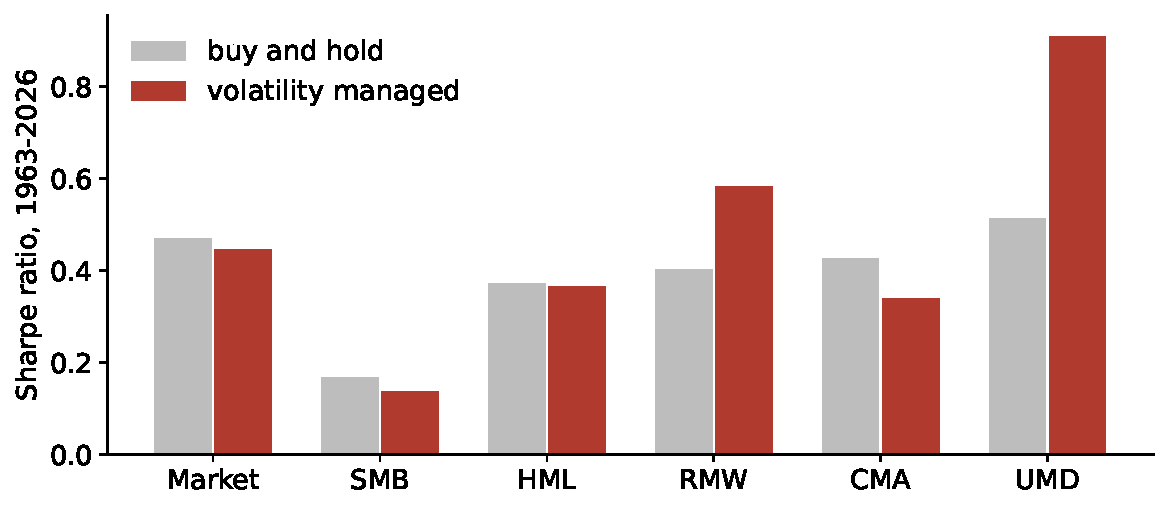
\includegraphics{figures/cs_factors.pdf}}
\end{column}
\begin{column}{0.44\textwidth}
\renewcommand{\arraystretch}{1.2}
\begin{tabular}{lccc}
\toprule
1963--2026 & before & after & alpha $t$ \\
\midrule
UMD & 0.51 & \textcolor{red}{0.91} & 5.9 \\
RMW & 0.40 & 0.58 & 3.4 \\
HML & 0.37 & 0.37 & 1.4 \\
Market & 0.47 & 0.45 & 1.4 \\
SMB & 0.17 & 0.14 & 0.2 \\
CMA & 0.43 & \textcolor{red}{0.34} & 0.6 \\
\bottomrule
\end{tabular}
\vskip 8pt
\begin{itemize}
\item Big for momentum, real for profitability
\vskip 4pt
\item Nothing, or worse, for the rest
\end{itemize}
\end{column}
\end{columns}
\end{frame}

\begin{frame}{It fails where volatile months are paid for}
\begin{center}
\adjustbox{max width=\textwidth, max height=0.56\textheight}{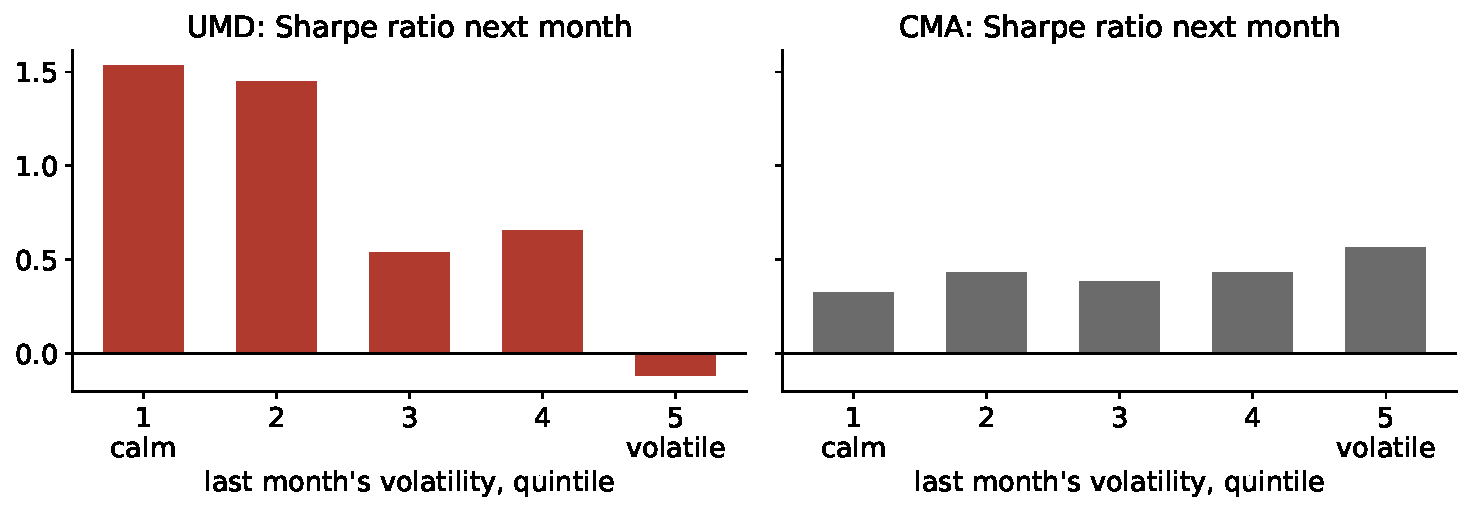
\includegraphics{figures/cs_sort_umd_cma.pdf}}
\end{center}
\begin{itemize}
\item UMD: Sharpe ratio 1.5 after the calmest months, \textcolor{red}{$-0.1$} after the most volatile. $b$ is about zero.
\vskip 4pt
\item CMA: higher after volatile months, 0.33 to 0.56. Its return rises with its risk: $b$ is large.
\vskip 4pt
\item Cutting CMA in volatile months cuts its best months. The formula on slide \ref{when} said so.
\end{itemize}
\end{frame}

\begin{frame}{Time the best mix, not just one factor}
First the tangency portfolio of the six factors, $W \propto \Sigma^{-1}\mu$, as in \emph{Capital Allocation I}. Then manage its volatility.
\vskip 6pt
\begin{center}
\renewcommand{\arraystretch}{1.3}
\begin{tabular}{lcc}
\toprule
the best mix of the six, same volatility & buy and hold & volatility managed \\
\midrule
1963--2026 & 1.17 & \textcolor{red}{1.28} \\
\quad 1963--1979 & 1.14 & 0.93 \\
\quad 1980--2014 & 1.34 & 1.63 \\
\quad 2015--2026 & 0.73 & 0.82 \\
\bottomrule
\end{tabular}
\end{center}
\vskip 6pt
\begin{itemize}
\item Alpha 2.2\% a year, $t = 5.4$. Sharpe ratio 2.0 after the calmest months, 0.85 after the most volatile.
\vskip 4pt
\item The weights use the whole sample, so the mix itself is in sample. The question is only whether timing it adds.
\vskip 4pt
\item Diversifying lowers the risk; timing the risk that is left still helps
\end{itemize}
\end{frame}

\begin{frame}{Why would risk be paid less when there is more of it?}
\vskip 6pt
\begin{itemize}
\item \textbf{Slow-moving capital.} When volatility jumps, leveraged traders must cut. Prices adjust, but slowly, and expected returns rise less than risk.
\vskip 10pt
\item \textbf{Crashes after rebounds.} Momentum is short the stocks that bounce back, and the bounce comes in volatile times (\emph{Momentum}).
\vskip 10pt
\item \textbf{Some investors do not react at all.} If most money is fixed, those who adjust can earn the difference.
\end{itemize}
\vskip 14pt
\begin{beamercolorbox}[rounded=true,sep=7pt,center]{box1}
These are hypotheses. The evidence is that it varies by factor, and by period.
\end{beamercolorbox}
\end{frame}

%================================================================== WHAT IT COSTS
\begin{frame}{Where it hurts: crashes out of calm, rebounds after storms}
\vskip 4pt
\begin{center}
\renewcommand{\arraystretch}{1.3}
\begin{tabular}{lccc}
\toprule
the market & weight that month & buy and hold & volatility managed \\
\midrule
October 1987 & 0.52 & $-23.1\%$ & $-12.0\%$ \\
October 2008 & 0.04 & $-17.2\%$ & $-0.7\%$ \\
March 2020 & 0.21 & $-13.4\%$ & $-2.9\%$ \\
April 2020 & \textcolor{red}{0.01} & \textcolor{red}{$+13.6\%$} & \textcolor{red}{$+0.2\%$} \\
\bottomrule
\end{tabular}
\end{center}
\vskip 10pt
\begin{itemize}
\item 1987 came out of a calm September, so the strategy was still half in
\vskip 6pt
\item After March 2020 it was out, and missed one of the best months in history
\vskip 6pt
\item It is a bet on persistence. A fast round trip is the worst case.
\end{itemize}
\end{frame}

\begin{frame}{The price: leverage}
\begin{center}
\adjustbox{max width=\textwidth, max height=0.50\textheight}{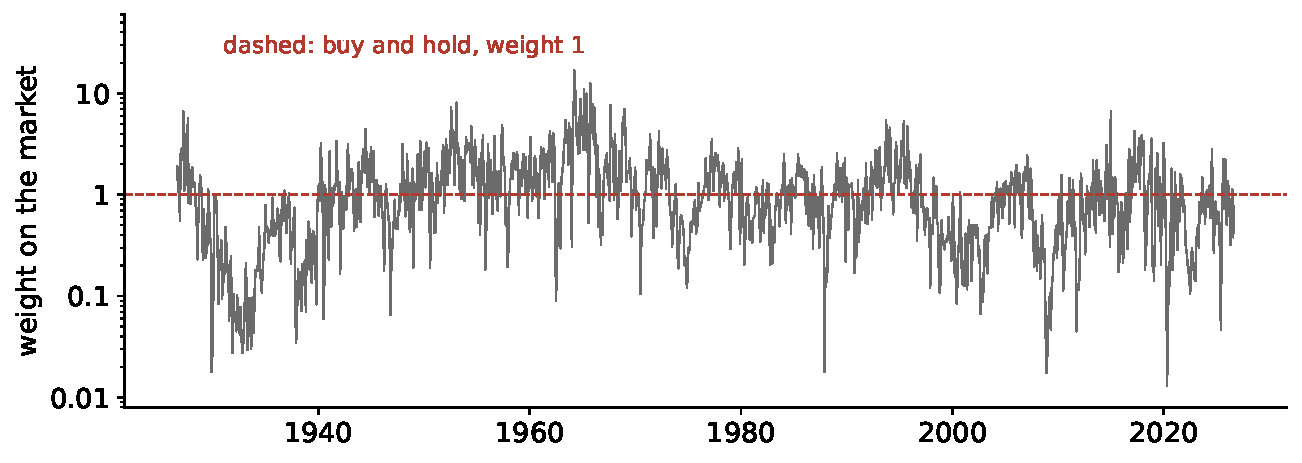
\includegraphics{figures/cs_weights.pdf}}
\end{center}
\begin{itemize}
\item Median weight 0.9. Above 2 in \textcolor{red}{16\%} of months. Largest, 16.9, in March 1964
\vskip 4pt
\item Capping the weight costs nothing here: Sharpe ratio 0.54 capped at 1, 0.55 at 2, against 0.52 uncapped
\vskip 4pt
\item The extreme weights come in the calmest months, where a calm month is easy to over-trust
\end{itemize}
\end{frame}

\begin{frame}{It trades, and a milder version does as well}
\vskip 6pt
\begin{itemize}
\item The weight moves by 0.74 a month on average: every month you buy or sell three-quarters of the position. Count the costs before you believe a small gain.
\vskip 10pt
\item Scale by $1/\sigma$ instead of $1/\sigma^{2}$: Sharpe ratio \textcolor{red}{0.56} against 0.52. It trades less and leans less on any one month.
\vskip 10pt
\item A dial again, as in \emph{Capital Allocation III}: from buy and hold ($1/\sigma^{0}$) to the full formula ($1/\sigma^{2}$)
\end{itemize}
\vskip 14pt
\begin{beamercolorbox}[rounded=true,sep=7pt,center]{box1}
In practice: volatility targets, risk budgets, and the stop-loss of \emph{Capital Allocation I}
\end{beamercolorbox}
\end{frame}

%================================================================== THE NOTEBOOK
\begin{frame}{Notebook, exercise 1: realized variance}
\vskip 4pt
\[ \text{RV}_{t} \;=\; \sum_{d \in t} \left(r_{d} - \bar r_{t}\right)^{2} \]
\vskip 4pt
\begin{itemize}
\item Daily market returns, 1926--2026. Group the days by month: \texttt{groupby(month)}
\vskip 6pt
\item For each month: its return, by compounding the days, and its RV
\vskip 6pt
\item Shift RV by one month, so each month carries the variance you knew when it started
\vskip 6pt
\item Plot the volatility. Measure how much of this month's volatility last month's explains, and how much of this month's \emph{return}
\end{itemize}
\vskip 10pt
\begin{beamercolorbox}[rounded=true,sep=7pt,center]{box1}
Look for: one correlation large, one about zero. Why \texttt{shift(1)}?
\end{beamercolorbox}
\end{frame}

\begin{frame}{Notebook, exercise 2: sort the months}
\vskip 4pt
\begin{itemize}
\item Put the months in five groups by last month's RV: \texttt{pd.qcut(rv\_lag, 5)}
\vskip 6pt
\item In each group, next month's volatility, average return and Sharpe ratio
\vskip 6pt
\item The full sample, 1926--2026: the same months as the sort on the slides
\end{itemize}
\vskip 14pt
\begin{beamercolorbox}[rounded=true,sep=7pt,center]{box1}
Look for: does the return rise with the volatility? Is $b$ closer to zero, or to one for one?
\end{beamercolorbox}
\end{frame}

\begin{frame}{Notebook, exercise 3: the volatility-managed market}
\[ r^{\sigma}_{t} \;=\; \frac{c}{\text{RV}_{t-1}}\; r_{t} \]
\vskip 2pt
From 1963, the years we have for all six factors. Three steps, two of them yours:
\vskip 6pt
\begin{enumerate}
\item \texttt{w\_raw = 1 / rv\_lag}
\vskip 4pt
\item \texttt{c}: the market's volatility over the volatility of \texttt{w\_raw * r}
\vskip 4pt
\item \texttt{managed = c * w\_raw * r}
\end{enumerate}
\vskip 6pt
Then compare Sharpe ratios, regress \texttt{managed} on the market for the alpha, and look at the weights.
\vskip 10pt
\begin{beamercolorbox}[rounded=true,sep=7pt,center]{box1}
Look for: the gain by period, and how large the weights get
\end{beamercolorbox}
\end{frame}

\begin{frame}{Notebook, exercise 4: all six factors}
\vskip 4pt
\begin{itemize}
\item The same three steps, in a loop over the six factors
\vskip 6pt
\item For each: Sharpe ratio before and after, the alpha and its $t$
\vskip 6pt
\item And the Sharpe ratio after the calmest 40\% of months against after the most volatile 40\%
\end{itemize}
\vskip 14pt
\begin{beamercolorbox}[rounded=true,sep=7pt,center]{box1}
Look for: which factors gain and which lose, and what the last two columns say about $b$
\end{beamercolorbox}
\end{frame}

\begin{frame}{Notebook, exercise 5: time the best mix}
\[ W \;=\; \Sigma^{-1}\mu \quad\longrightarrow\quad r^{\text{mix}}_{d} = W' r_{d} \quad\longrightarrow\quad \frac{c}{\text{RV}^{\text{mix}}_{t-1}}\; r^{\text{mix}}_{t} \]
\vskip 4pt
\begin{enumerate}
\item The tangency weights from the monthly returns of the six factors: invert the covariance matrix, times the means
\vskip 4pt
\item The mix's \emph{daily} return, so it has a realized variance of its own
\vskip 4pt
\item The same three steps as exercise 3, on the mix
\end{enumerate}
\vskip 10pt
\begin{beamercolorbox}[rounded=true,sep=7pt,center]{box1}
Look for: does timing still add once the factors already diversify each other?
\end{beamercolorbox}
\end{frame}

\begin{frame}{Takeaways}
\begin{enumerate}
\item The formula has two parts that move. Volatility is easy to forecast; expected returns are not.
\vskip 4pt
\item Last month's realized variance is a crude forecast of next month's, and hard to beat by much.
\vskip 4pt
\item Holding less after volatile months pays only if the return does not rise with the risk.
\vskip 4pt
\item It pays a lot for momentum and for the best mix, some for profitability. For the market it depends on the period; for CMA it hurts.
\vskip 4pt
\item Its worst case is a fast round trip. It needs leverage and it trades; caps and milder scaling give up little.
\end{enumerate}
\vskip 10pt
\begin{beamercolorbox}[rounded=true,sep=7pt]{box1}
\textbf{Homework: cap the leverage.} Volatility-manage momentum with the weight capped at 2. One number, three sentences.
\end{beamercolorbox}
\end{frame}

%================================================================== APPENDIX
\appendix
\begin{frame}
\begin{center}
{\Large Appendix}
\end{center}
\end{frame}

\begin{frame}[label=appendix_rv]{A1: How the managed strategy is built}
\begin{itemize}
\item \textbf{Realized variance}: $\text{RV}_{t} = \sum_{d \in t} (r_{d} - \bar r_{t})^{2}$, over the trading days $d$ of month $t$. Times 12 is a variance a year.
\vskip 8pt
\item \textbf{The weight}: $c/\text{RV}_{t-1}$ uses only last month's days, so it is known before month $t$ starts.
\vskip 8pt
\item \textbf{The constant} $c$ uses the whole sample, so the strategy as written could not have been run. But $c$ only scales every weight by the same number: it changes no Sharpe ratio and no $t$-statistic. In real time, target a volatility instead.
\vskip 8pt
\item The same construction as volatility-managed momentum in \emph{Momentum}.
\end{itemize}
\hfill \hyperlink{managed}{\beamerreturnbutton{Back}}
\end{frame}

\begin{frame}{A2: Data, and what to be careful about}
\begin{itemize}
\item \textbf{Market, 1926--2026.} Ken French's daily market factor. The six factors daily from 1963.
\vskip 8pt
\item \textbf{No costs.} The managed strategy trades every month and runs leverage. Both cost money, and borrowing costs more than T-bills.
\vskip 8pt
\item \textbf{One rule, chosen afterward.} Sorting into five groups and scaling by last month's variance are standard, but the periods and factors where it works were found by looking.
\vskip 8pt
\item \textbf{Periods differ.} The market gains in 1926--1945 and 1980--2014, and loses in 1946--1979 and 2015--2026.
\vskip 8pt
\item \textbf{The holding-period table} uses blocks of trading days, not calendar months, so its monthly row differs slightly from the rest.
\end{itemize}
\end{frame}

\end{document}
